\documentclass{article}
\usepackage[utf8]{inputenc}
\usepackage{mathpazo} % Palatino font
\usepackage{natbib}
\usepackage{graphicx}
\usepackage{enumitem}
\usepackage{amsmath}
\usepackage{amssymb}
\usepackage{ragged2e}
\usepackage{subfig}
\usepackage{algorithm}
\usepackage{algorithmic}
\usepackage{diagbox}
\usepackage[textwidth=12.7cm]{geometry}


\usepackage{xcolor}
\newcommand\todo[1]{\textcolor{red}{#1}}

\bibliographystyle{abbrv} %format des citations

\begin{document}
\begin{titlepage}
	\newcommand{\HRule}{\rule{\linewidth}{0.5mm}}
					
	\center
					
	\textsc{\LARGE Université de Bordeaux}\\[1.5cm]
					
	\textsc{\Large Master 1 Informatique}\\[0.5cm]
					
	\textsc{\large Projet de programmation}\\[0.5cm]
					
	\HRule\\[0.4cm]
					
	{\huge\bfseries Génération de playlistes musicales pour un groupe d'utilisateurs}\\[0.4cm]
	{\Large\bfseries Mémoire}
	\HRule\\[1.5cm]
					
	\begin{minipage}{0.4\textwidth}
			
		\begin{flushleft}
			\large
			\textit{Client}\\
			\textsc{Hanna}  Pierre 
		\end{flushleft}
				
		\begin{flushleft}
			\large
			\textit{Chargés de TD}\\
			\textsc{Boussicault}  Adrien 
			\textsc{Narbel}  Philippe 
		\end{flushleft}
				
		\begin{flushleft}
			\large
			\textit{Auteurs}\\
			\textsc{Bah} Elhajd Amadou
			\\
			\textsc{Deguillaume} Nicolas
			\\
			\textsc{Jolliet} Louis
			\\
			\textsc{Loison} Jules 
			\\
			\textsc{Vigneau} Paul 
		\end{flushleft}
				
	\end{minipage}
	\vfill\vfill\vfill
					
	{\large 6 Avril 2020}
	\vfill\vfill
	
\includegraphics[width=0.5\textwidth]{ressources/Logo.jpg}\\[1cm]
		\vfill
		\end{titlepage}
		\justify
		\renewcommand{\contentsname}{Table des matières}
		\tableofcontents
		\newpage
								
		\section{Contexte}
    	\subsection{Résumé}
    	\paragraph{}
    	Lorsqu'un groupe de personnes écoute de la musique - par exemple, lors d'un trajet en voiture - il est fréquent que le monopole de la musique soit détenu par le propriétaire de l'appareil diffusant cette dernière. Ce projet vise à répondre à un besoin précis : à l'aide d'un logiciel permettant de connecter plusieurs utilisateurs d'un service de streaming musical, être capable de proposer à l'aide d'algorithmes un ensemble de musiques susceptible de satisfaire l'ensemble des personnes présentes.
    	
    	\subsection{Introduction du projet}
		\paragraph{}
		Notre client souhaite une application permettant de résoudre un problème lié à l'écoute de musique entre plusieurs personnes. En effet, il constate que lorsque plusieurs utilisateurs veulent écouter de la musique au même endroit, il n'y a pas d'autre choix que d'utiliser le compte d'un seul de ces utilisateurs, et donc d'imposer les goûts de cet utilisateur aux autres personnes présentes.
		
		Le client propose donc comme solution une application ayant pour objectif de générer des playlists de titres musicaux basées sur les écoutes et les goûts de chaque utilisateur connecté à l'application. Les données seront récupérées auprès des API de Spotify ou Deezer, deux services populaires de streaming musical.
		
    	L'intérêt principal de ce projet est de créer un produit qui puisse être utilisé par des chercheurs du LaBRI. En effet, il s'agit en particulier de faire de la recherche sur des algorithmes de recommandation musicale auprès d'utilisateurs. Une partie de notre travail sera donc de réfléchir et d'implémenter des algorithmes visant à générer des playlists musicales. Pour cela, l'application devra récupérer les informations d'écoute de ces utilisateurs (musiques appréciées, playlists personnelles, genres les plus écoutés, etc). 
    	
    	En plus de la génération de playlist, l'application devra permettre à l'utilisateur d'écouter cette playlist, en embarquant un lecteur de musique comprenant des options basiques telles que le changement de musique, la mise en pause et la reprise de l'écoute, pouvoir mettre un "j'aime", etc. Toutes ces actions devront être enregistrées sous formes de logs d'écoute afin de pouvoir analyser et évaluer les différents algorithmes proposés. Une fois l'application produite, les chercheurs du LaBRI pourront ensuite ajouter et analyser de nouveaux algorithmes adaptés à leurs besoins.
								
		Concernant le service de streaming utilisé, nous avons choisi d'utiliser l'API de Spotify dans un premier temps car nous sommes plus familiers avec ce service.
								
		\subsubsection{Descriptions des termes}
		\begin{itemize}
		    \item Plateforme / Plateforme de streaming : site internet d’hébergement de musique en ligne qui permet à ses utilisateurs de pouvoir écouter une musique instantanément. (Spotify, Deezer)
			\item Track (Morceau): morceau de musique
			\item Playlist (Liste de lecture) : liste de morceaux de musique. Dans ce document on ajoutera souvent un adjectif à la suite du mot \textit{playlist} parmi les suivants : 
			      \begin{itemize}
			      	\item Personnelle : playlist enregistrée sur le compte d'un utilisateur en particulier.
			      	\item Locale : playlist créée sur notre application et qui n'existe que dans celle-ci. Elle n'existe sur aucun compte utilisateur (Spotify ou Deezer).
			      	\item Publique : visibilité d'une playlist personnelle. Le contenu de la playlist est accessible par tout le monde.
			      	\item Privée : visiblité d'une playlist personnelle. La playlist et son contenu n'est accessible que par l'utilisateur qui a créé et enregistré cette playlist sur une plateforme de streaming.
			      \end{itemize}
			\item Utilisateur : personne physique détentrice d'un compte Spotify ou Deezer. Un ensemble d'utilisateur constitue un groupe.\newline
			Dans ce document on ajoutera souvent un adjectif à la suite du mot \textit{utilisateur} parmi les suivants:
			      \begin{itemize}
			      	\item Authentifié ou principal (main user) : utilisateur qui a autorisé notre application à utiliser son compte Spotify ou Deezer afin d'effectuer des requêtes.
			      	\item Utilisateur courant (current user) : utilisateur qui a l'appareil en main et qui s'est désigné comme celui qui interagit avec l'application.
			      	\item Utilisateur secondaire (other user) : utilisateur qui a renseigné son nom d'utilisateur afin de s'ajouter au groupe.
			      \end{itemize}
			\item Session d'écoute : moment durant lequel les titres de la playlist locale sont en écoute
		\end{itemize}
		
		\subsubsection{Acteurs}
		\begin{itemize}
			\item Utilisateurs: principal, secondaires ou courants, ils utilisent et interagissent avec l'application
			\item Serveur Spotify : serveur que l'on sollicite via l'API afin d'accéder aux informations des utilisateurs ainsi qu'à des fonctionnalités comme la création de playlists personnelles ou la modification de celles-ci 
		\end{itemize}

		\subsection{Description et analyse de l'existant}
		\subsubsection{Services similaires}
		\paragraph{}
		Nous démarrons notre application de zéro, cependant il existe certains exemples nous permettant d'avoir des idées de fonctionnalités ou de design. Pour le moment, les seuls exemples dont nous pouvons nous inspirer qui correspondent le plus à ce que nous devons réaliser sont Friends Mix par Apple et Family Mix par Spotify. En effet, Apple Music propose un mix, renouvelé chaque semaine incluant les 25 chansons les plus écoutées par nos amis. De la même façon, Spotify, dans leur offre Premium Family (pouvoir avoir jusqu'à 6 utilisateurs sur un même compte), offre une playlist incluant les goûts de chacun. Ces applications possèdent un certain nombre des fonctionnalités énoncées en \ref{besoins}, mais il est bien sûr impossible de customiser l'algorithme de génération des playlists, ce qui est le but premier de notre client. Ces algorithmes sont propriétéaires et sont donc privés, nous devrons donc nous intéresser à des sources externes (cf. \ref{algos})Nous pouvons cependant nous inspirer de certaines fonctionnalités disponibles et pouvons améliorer l'expérience utilisateur, tel que la provenance des musiques (de quel(s) utilisateur(s) provient la musique) comme on peut le voir sur la Figure \ref{fig:example_app}.
		De plus nous allons nous servir de différents dépots GitHub utilisant les API Spotify \cite{spotify-web-api} ou Deezer.
								
		\begin{figure}[hb!]
			\centering
			\subfloat[Friends Mix - Apple Music]{{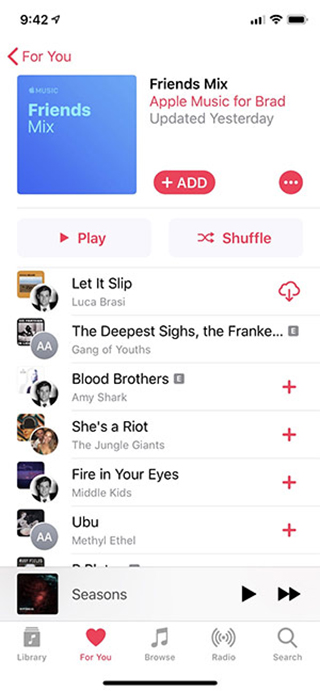
\includegraphics[width=5cm]{ressources/friends-mix-apple-music.jpg} }}%
			\qquad
			\subfloat[Family Mix - Spotify]{{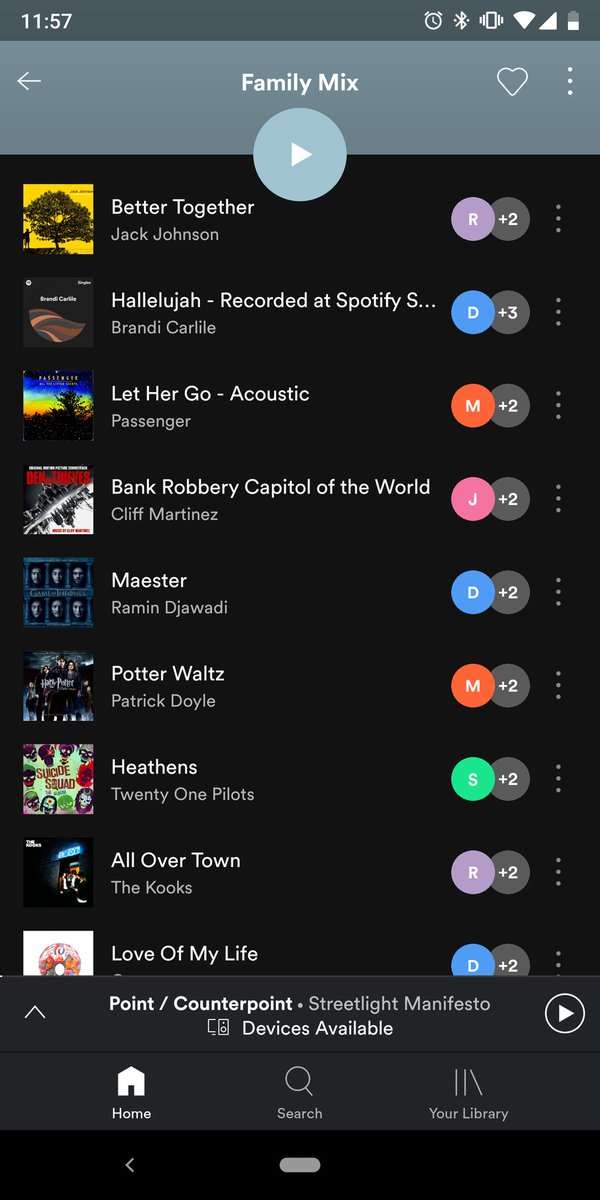
\includegraphics[width=5cm]{ressources/Spotify_Family_Mix.jpg} }}%
			\caption{Exemple d'applications similaires}%
			\label{fig:example_app}%
		\end{figure}
		
		\subsubsection{Algorithmes de génération de playlist}\label{algos}
    	\todo{TODO}

% 		\subsubsection{Calcul du score}
		
% 		\subsubsection{Least Misery Strategy}
		

		\subsection{Exemples de base}

        \subsubsection{Interface utilisateur}\label{interface_utilisateur}
            	En nous inspirant des visuels présentés précédemment (Figure \ref{fig:example_app}) nous avons imaginé les prototypes d'interface ci-dessous (Figure \ref{fig:gui}). C'est une interface assez simpliste, qui permet d'accéder à toutes les fonctionnalités rapidement. Cette interface peut être divisée en plusieurs parties. En haut on peut accéder aux fonctionnalités qui ne sont pas directement liées à la musique comme les paramètres. Ensuite il y a la partie permettant de visualiser la playlist locale. Les lettres associées aux titres correspondent aux utilisateurs d'où provient le titre en question.
            	Enfin, on peut voir en bas le "player" qui permet de gérer la lecture des titres, avec leur pochette visible à gauche.
		\begin{figure}[hb!]
			\centering
			\subfloat[Page de connexion]{{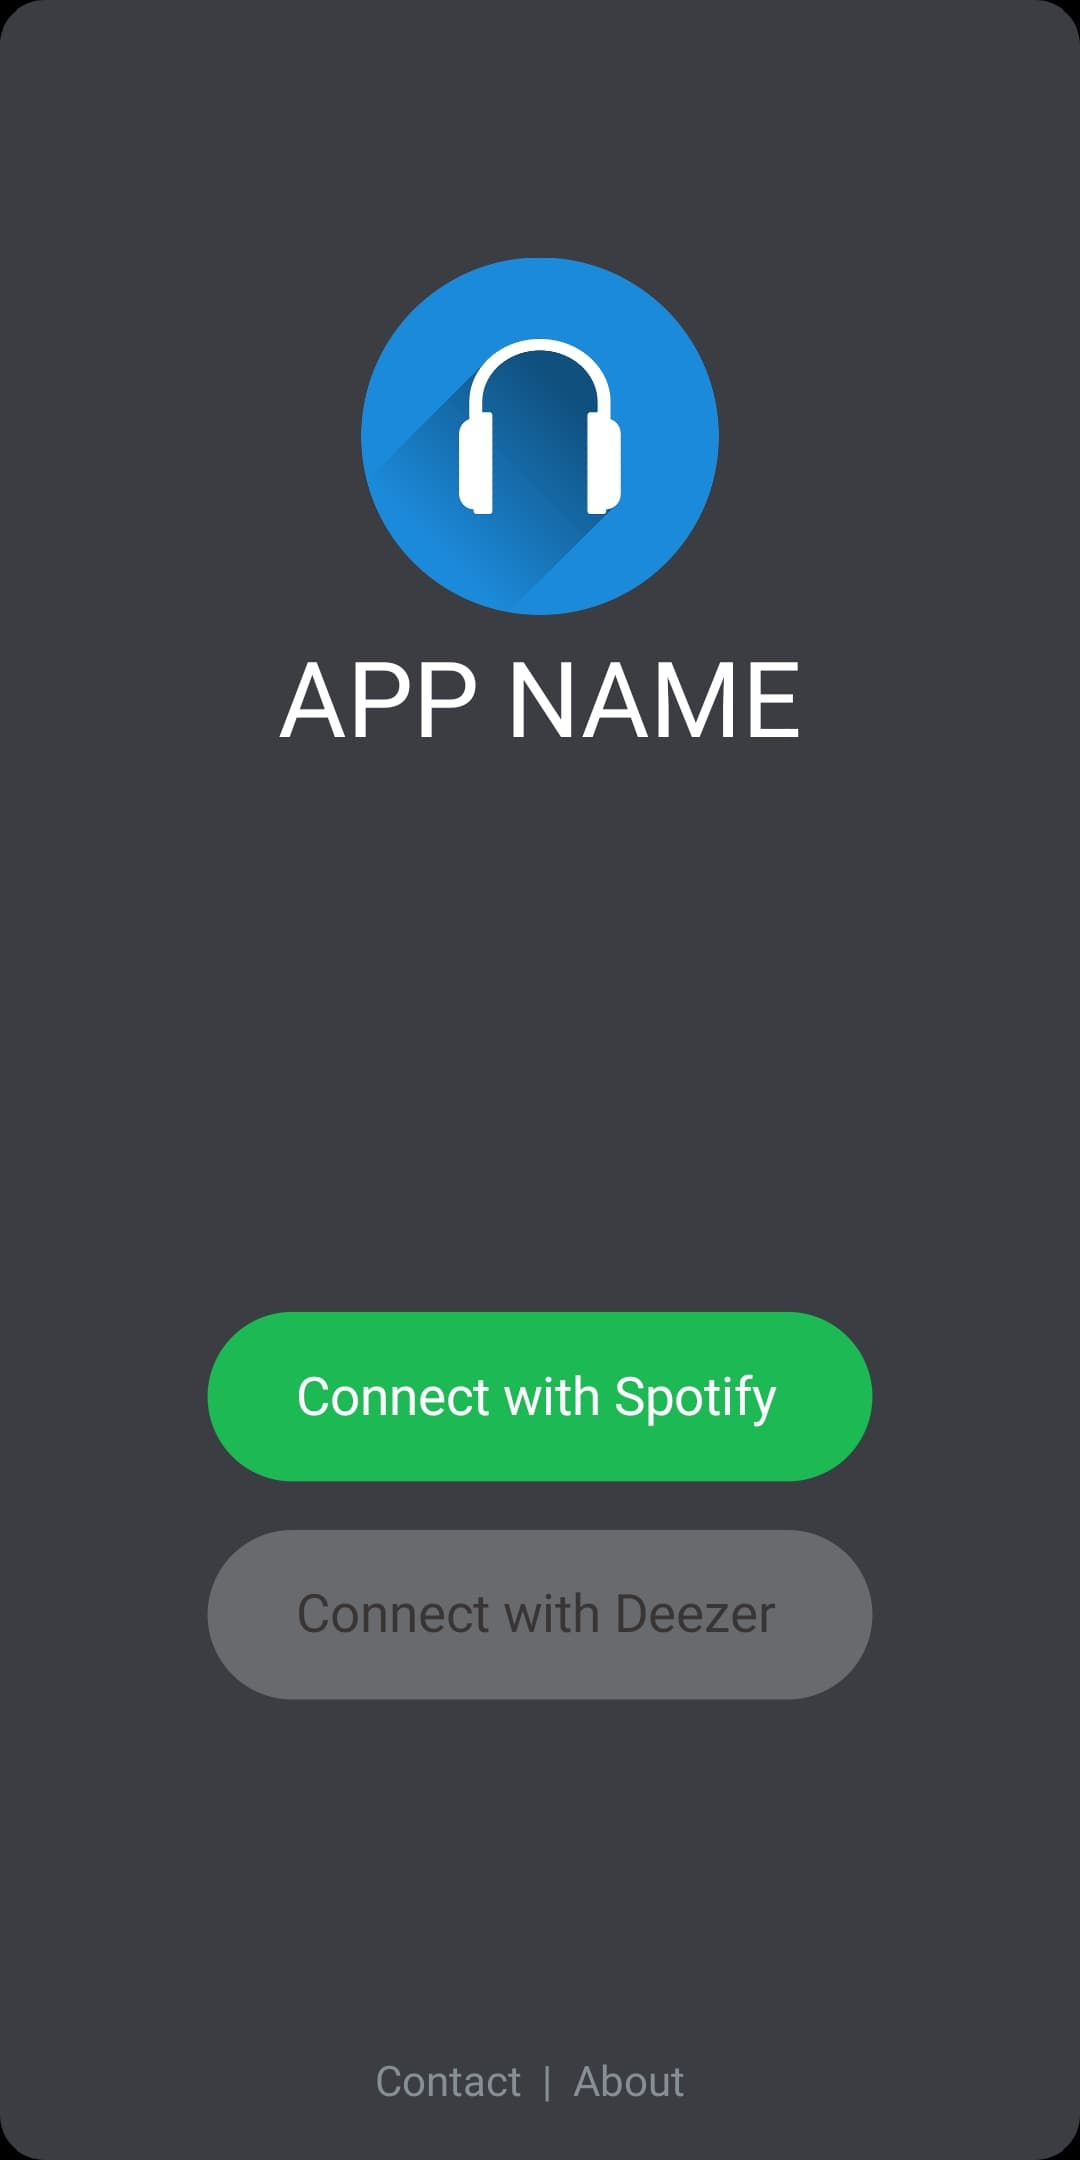
\includegraphics[width=4cm]{ressources/connection_page.jpg} }}\label{test}
			\subfloat[Page principale]{{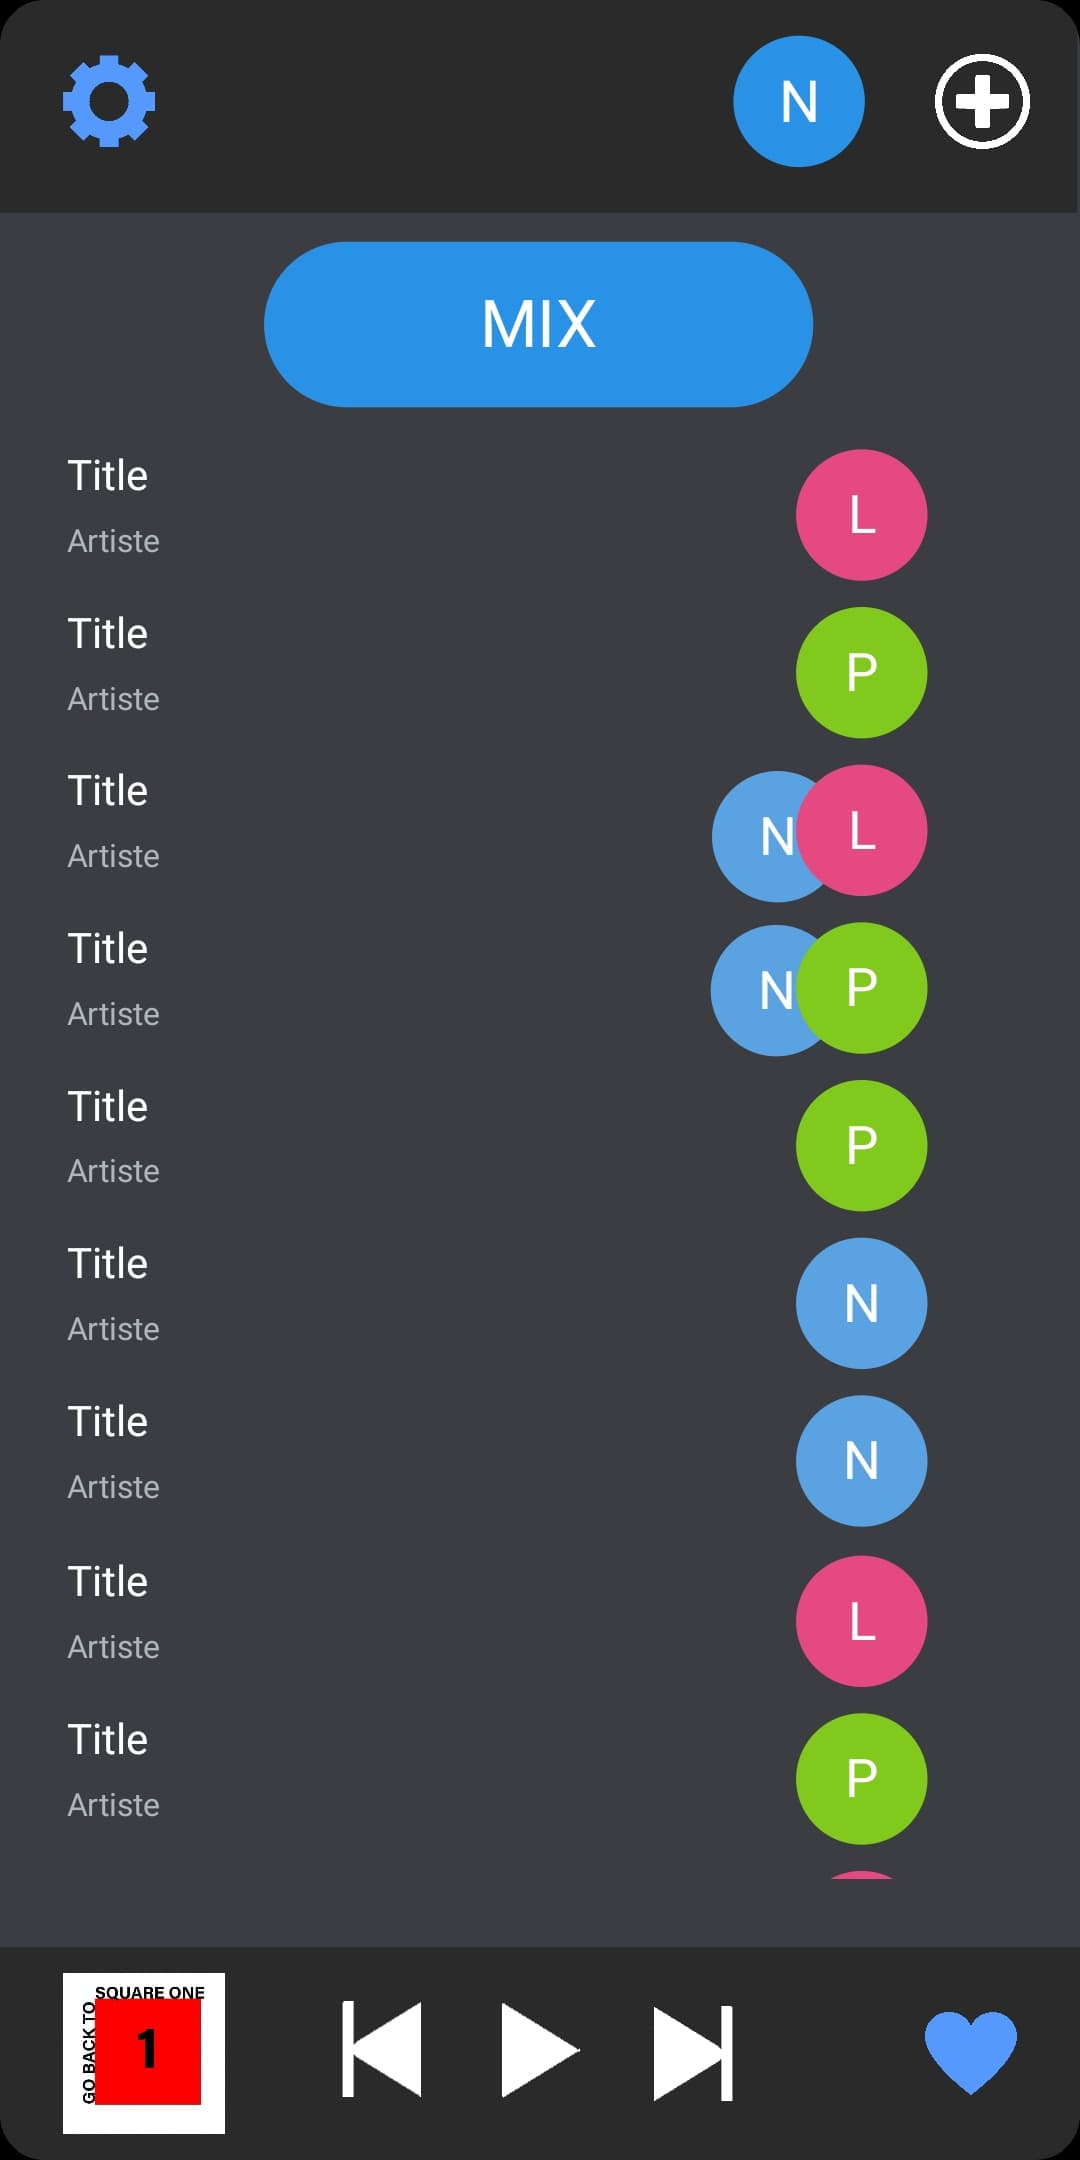
\includegraphics[width=4cm]{ressources/home_page.jpg} }}
			\caption{Prototypes d'interface utilisateur}
			\label{fig:gui}
		\end{figure}
        \subsubsection{Cas global d'utilisation}\label{interface_utilisateur}
    	\todo{TODO des exemples choisis qui permettent
                d'illustrer l'introduction et la description du projet (et ce n'est pas
                nécessairement une sous-partie).
                }
                \newpage		
		\section{Description des besoins} \label{besoins}
		Afin de décrire la priorité de chaque besoin, nous écrirons au début de la description d'un besoin un de ces mots :
		\begin{itemize}
			\item \textbf{Essentiel} : le logiciel ne sera pas acceptable sans que ce besoin ne soit réalisé
			\item \textbf{Conditionnel} : besoin qui étend et améliore le logiciel, sans que ce besoin soit nécessaire pour rendre le logiciel acceptable
			\item \textbf{Optionnel} : besoin dont la valeur n’est pas encore assurée. Donne au fournisseur l’occasion de proposer quelque chose qui va au-delà des besoins attendus
		\end{itemize}
		\subsection{Besoins fonctionnels}
		Nous détaillerons les besoins suivants, exprimés par le client :
		\subsubsection{Choisir une plateforme de streaming musical sur laquelle s'interfacer}
		\textbf{[ Essentiel ]}
		\begin{itemize}
			\item Pouvoir choisir d'utiliser l'API de Spotify au démarrage de l'application
		\end{itemize}
		\textbf{[ Optionnel ]}
		\begin{itemize}
			\item Pouvoir choisir d'utiliser l'API de Deezer au démarrage de l'application
		\end{itemize}
		\subsubsection{Authentifier l'utilisateur principal} \label{authentification}
		\textbf{[ Essentiel ]}
		\begin{itemize}
			\item Après avoir choisi quelle API utiliser, un utilisateur doit pouvoir s'authentifier
		\end{itemize}
		\textbf{Test du besoins} 
		\begin{itemize}
			\item On s'authentifie au début du test. On vérifie ensuite que l'authentification s'est bien passée ainsi que le bon fonctionnement des requêtes. Pour cela nous envoyons la requête suivante: \textit{GET https://api.spotify.com/v1/me} pour récupérer le profil de l'utilisateur authentifié. On regarde ensuite le code de retour de la requête. Si le code de retour est 200, cela signifie que la requête a réussi et que donc l'authentification aussi (car cette requête récupère les informations de l'utilisateur authentifié). Si le code de retour est 401, cela signifie que l'authentification a échouée
		\end{itemize}
		\newpage
		\subsubsection{Créer un groupe d'utilisateurs}
		\textbf{[ Essentiel ]}
		\begin{itemize}
			\item Réussir l'authentification crée un groupe d'utilisateurs contenant intialement seulement l'utilisateur principal
		\end{itemize}
		\subsubsection{Ajouter des membres secondaires au groupe}  \label{connexion}
		\textbf{[ Essentiel ]}
		\begin{itemize}
			\item Cliquer sur un bouton et renseigner un identifiant utilisateur dans une boîte de texte permet d'ajouter un utilisateur au groupe
		\end{itemize}
		\textbf{Test du besoin} 
		\begin{itemize}
			\item On renseigne des identifiants utilisateur (id) au début du test. Pour chaque id renseigné, on envoie la requête \textit{GET https://api.spotify.com/v1/users/\{id\}} pour récupérer le profil de chaque utilisateur. On regarde ensuite le code de retour de la requête. Si le code de retour est 200, cela signifie que la requête a réussi: le test réussit. Si le code de retour de la requête est 404, cela signifie que l'utilisateur n'existe pas, le test échoue
		\end{itemize}
		\subsubsection{Supprimer des membres du groupe}
		\textbf{[ Essentiel ]}
		\begin{itemize}
			\item Supprimer l'utilisateur principal le fera se déconnecter et supprimera la session d'écoute et le groupe
		\end{itemize}
		\textbf{[ Conditionnel ]}
		\begin{itemize}
			\item Un utilisateur secondaire doit pouvoir être supprimé du groupe
		\end{itemize}
						            
		\subsubsection{Ignorer un utilisateur dans la génération de playlist}
		\textbf{[ Conditionnel ]}
		\begin{itemize}
			\item Un utilisateur doit pouvoir être ignoré dans l'algorithme (fonction "mute") : ses données ne seront pas utilisées pour le calcul de la playlist locale (cf. \ref{interface_utilisateur} (c))
		\end{itemize}
		\subsubsection{Accès aux informations de chaque utilisateur} 
		Une fois un utilisateur ajouté au groupe (cf. \ref{authentification} ou \ref{connexion}), il faut accéder à ses chansons préférées via l'API choisie. 
		\newline \\
		\textbf{[ Essentiel ]}
		\begin{itemize}
			\item Récupérer et charger en mémoire les playlists publiques des utilisateurs au format JSON via l'API
		\end{itemize}
		\textbf{Test du besoin}
		\begin{itemize}
			\item On s'authentifie et on renseigne des identifiants utilisateur (id) au début du test. Pour chaque id renseigné, on envoie la requête \newline\textit{GET https://api.spotify.com/v1/users/\{id\}/playlists} pour récupérer les playlists de chaque utilisateur. Si le code de retour de la requête est 404, cela signifie que l'utilisateur n'existe pas: le test échoue. Si le code de retour de la requête est 200, on continue le test. On envoie ensuite la requête \textit{ GET https://api.spotify.com/v1/me/playlists} pour récupérer les playlists de l'utilisateur authentifié. Si le code de retour de la requête est 200 le test réussit, sinon le test échoue. \newline
			      Tous les tests qui nécessitent les playlists les récupèrent au début du test de la même manière que dans ce test
		\end{itemize}
		\textbf{[ Conditionnel ]} \label{connexion de tous les utilisateurs}
		\begin{itemize}
			\item Récupérer et charger en mémoire d'autres informations (sous format JSON) comme les chansons aimées ou les artistes préférés.\\
			Cependant, ces informations sont privées, cela nécessite d'implémenter une connexion de tout les utilisateurs. Il faut donc, au moment d'ajouter un utilisateur, lui proposer de s'authentifier auprès de Spotify (et donc de ne plus lui demander son identifiant) - comme pour la connexion du premier utilisateur. Cette connexion va permettre de récupérer un jeton propre à la connexion qui permettra par la suite d'effectuer des requêtes afin de récupérer les informations privées du compte.\\
			Néanmoins, l'écoute de la musique doit se faire depuis un compte premium, qui sera celui de la première personne à se connecter à l'application, au moment de l'ouverture.\\
			Cette solution n'est qu'une supposition de ce qu'il est possible de faire. Il n'y a eu aucun prototype visant à tester cette fonctionnalité.
		\end{itemize}
		\subsubsection{Proposition de playlist(s)}
		\textbf{[ Essentiel ]}
		\begin{itemize}
			\item L'application devra pouvoir créer une playlist vide
			\item L'application devra pouvoir ajouter les titres retournés par l'algorithme à cette playlist locale
			\item L'utilisateur doit pouvoir lancer un mix (génération de playlist) : ce qui aura pour effet de lancer l'algorithme puis lancer automatiquement l'écoute de la première chanson de la playlist locale générée par ce dernier
		\end{itemize}
		\textbf{Test des besoins}
		\begin{itemize}
			\item On s'authentifie, on renseigne des identifiants utilisateur (id) et on récupère les playlists des utilisateurs au début du test. On crée une playlist, représentée par une structure de données sur laquelle on effectue un test pour savoir si elle est de taille 0 si c'est le cas le test continue, dans le cas contraire il échoue. On fait tourner l'algorithme de génération de playlist. On ajoute ces titres à la structure de données représentant la playlist. On teste si la taille de la playlist est de taille \textit{n} (\textit{n} étant le nombre de musiques générées). Si c'est le cas, le test réussit, sinon il échoue
		\end{itemize}
		\textbf{[ Optionnel ]}
		\begin{itemize}
			\item Pouvoir ajouter les playlists au compte Spotify de l'utilisateur principal
			\item Pouvoir renseigner sur l'application des données qui seront incluses à la requête de création de playlist personnelle : 
			      \begin{itemize}
			      	\item Nom : renseigne le nom de la playlist (chaîne de caractères)
			      	\item Visibilité : définit si la playlist est privée ou publique (booléen, \textit{true} pour publique et \textit{false} pour privée)
			      	\item Collaboration : définit si la playlist est collaborative ou pas (booléen). Pour qu'une playlist soit collaborative, il faut qu'elle soit privée.
			      	\item Description : renseigne la description de la playlist (chaîne de caractères)
			      \end{itemize}
		\end{itemize}
		\textbf{Test du besoin}
		\begin{itemize}
			\item On s'authentifie, on renseigne des identifiants utilisateur (id) et on récupère les playlists des utilisateurs au début du test. On envoie la requête \textit{POST https://api.spotify.com/v1/users/\{id\}/playlists} pour créer une playlist sur le compte de l'utilisateur authentifié (id doit donc être son identifiant utilisateur). On envoie ensuite les requêtes \textit{POST https://api.spotify.com/v1/playlists/\{playlist\_id\}\newline/tracks} en renseignant l'identifiant des musiques à ajouter. Si le code de retour des requêtes est 200 le test réussit, sinon le test échoue.
		\end{itemize}
		\subsubsection{Proposer différents algorithmes de génération de playlists}
		\textbf{[ Essentiel ]}
		\begin{itemize}
			\item  L'application implémentera un algorithme naïf qui proposera des musiques prises au hasard dans les playlists publiques des utilisateurs.\newline \\
			      Le premier algorithme que nous allons implémenter est un algorithme de test, dit naïf qui sera utilisé pour tester l'achitecture que nous avons choisie (cf. \ref{archi_log}). Il consistera à récupérer un nombre égal de musiques provenant des playlists publiques de chaque utilisateur, sans critère particulier. Ce nombre sera défini comme la taille maximale d'une playlist locale (cf. \ref{performance}) divisée par le nombre d'utilisateurs.
			      		
		      \item  L'application proposera au moins un algorithme \cite{ICDM2017} permettant de tester les fonctionnalités proposées par le produit final.\newline \\
		            Le premier algorithme à implémenter consiste à analyser les chansons des playlists publiques grâce au service \textit{Audio Features and Analysis} de l'API Spotify \cite{spotify-web-api}. Celle-ci permet d'obtenir des données sur une chanson comme son degré d'acoustique, son tempo, son énergie, etc. Nous allons par la suite analyser ces données \cite{Data_analysis} en effectuant les opérations suivantes : 
		            \begin{itemize}
		                \item Profil type de chaque utilisateur en effectuant la moyenne des données de chaque titre sous forme de vecteur
		                \item Observer la diversification des utilisateurs (est-ce qu'un utilisateur écoute des musiques diversifiées selon les données) 
		            \end{itemize}
		            Cela permet de mettre en valeur les données les plus importantes pour chaque utilisateur. Par la suite, on compare le profil type de chaque utilisateur sur toutes les musiques de toutes les playlists. Pour faire cela, on calcule la différence terme à terme entre les données du profil d'un utilisateur et les données d'une musique. Cela nous donne un vecteur que nous transformons en une valeur en utilisant la formule de la distance euclidienne. La valeur calculée est le score d'une musique pour un utilisateur. On calcule donc cette valeur pour chaque musique pour chaque utilisateur. \\
		            Par la suite, on attribut un score final à chaque musique en utilisant la \textit{Least Misery Strategy} \cite{Masthof2011} qui est une stratégie d'évaluation qui évalue un item avec le plus bas score qu'un utilisateur lui a attribué. De cette façon, il n'y aura pas de chanson détestée par un utilisateur dans la playlist générée.
			      
			\item L'application proposera de changer d'algorithme dans les options (car le client pourra ajouter des algorithmes)
		\end{itemize} 
		\textbf{[ Essentiel ]}
		\begin{itemize}
			\item  L'application proposera d'autres algorithmes \cite{ICDM2017} plus complexes permettant une réelle analyse des données. \newline \\
			      Le second algorithme que nous implémenterons se base sur un autre article scientifique \cite{Masthof2011} qui met en avant la notation des éléments pour déterminer comment les proposer à un groupe d'utilisateurs. Cet algorithme nécessite la réalisation du besoin fonctionnel conditionnel d'authentification de tous les utilisateurs (cf. \ref{connexion de tous les utilisateurs}) pour être implémenté. \newline
			      Spotify ne propose pas de système de notation des chansons pour chaque utilisateur. Il nous faut donc attribuer nous même un score à chaque titre en fonction des données récupérées des utilisateurs. On récupère les 50 (limite de la requête) titres les plus écoutés de chaque utilisateur. On cherche ensuite à affecter un score à chacun des titres en fonction de plusieurs critères : 
			      \begin{itemize}
			      	\item Classement des titres en terme d'écoute
			      	\item Si un titre est dans la liste des titres préférés d'autres utilisateurs
			      	\item Si un titre dans la liste d'un utilisateur a le même artiste qu'un titre de la liste d'un autre utilisateur (et que les titres ne sont pas les mêmes)
			      \end{itemize}
			      Une fois ce classement terminé, on a au plus \textit{50 * nombre d'utilisateurs dans le groupe} titres à partir desquels créer la playlist locale. On sélectionne les \textit{x} premiers titres qui ont le score le plus élevé. Avec \textit{x} étant la taille maximale de la playlist locale (cf. \ref{performance}).
		\end{itemize}
		\subsubsection{Lecture de la playlist locale, avec possibilité de skipper des titres} \label{lecture}
		\textbf{[ Essentiel ]} 
		\begin{itemize}
			\item L'utilisateur pourra écouter des chansons et pourra effectuer les interactions suivantes :
			      \begin{itemize}
			      	\item Resume/pause
			      	\item NextTrack/previousTrack
			      	\item Like
			      \end{itemize}
		\end{itemize}
		\textbf{Tests du besoin}
		\begin{itemize}
			\item On s’authentifie. On initialise le lecteur (SDK). On ajoute un \textit{EventListener} sur l'évènement \textit{ready} et sur l'évènement \textit{not\_ready}. Si le premier évènement est déclenché on peut continuer le test, si le second l'est le test échoue. On ajoute un \textit{EventListener click} sur le bouton \textit{like} et sur l'évènement \textit{player\_state\_changed} qui est appelé dès que l'état du lecteur change, l'API nous retourne alors un objet contenant diverses informations sur la session. On lance 3 musiques. On met en pause, on vérifie que la variable \textit{paused} est \textit{true}. On relance la musique, on vérifie que la variable \textit{paused} est \textit{false}. On vérifie que la musique jouée est la 1ère des 3. On vérifie que la musique suivante est la 2ème. On accède à la musique suivante. On vérifie que la musique actuelle est la 2ème, que la musique précédente est la 1ère et que la suivante est la 3. On accède à la musique précédente. On vérifie que la musique actuelle est la 1 et que la musique suivante est la 2. On  \textit{like} le titre. On vérifie que l'on est bien passé dans l'évènement du \textit{like}. Si toutes les vérifications sont passées, c'est que le test réussit. Si une vérification ne passe pas, le test échoue
		\end{itemize}
		\textbf{[ Conditionnel ]}
		\begin{itemize}
			\item L'utilisateur courant est visible en haut de l'application (cf. \ref{interface_utilisateur} (b)) 
			\item L'utilisateur physique pourra choisir qui est l'utilisateur courant (pour pouvoir associer les interactions précédemment énoncées à un utilisateur). Pour cela il devra cliquer sur l'icône utilisateur, puis sélectionner l'utilisateur courant. Cela aura pour utilité d'identifier l'utilisateur qui interagit avec l'application
		\end{itemize}
		\textbf{[ Optionnel ]}
		\begin{itemize}
			\item L'utilisateur pourra se déplacer dans une chanson via une pop-up qui s'affichera en cliquant sur la chanson en cours. 
			\item Cette pop-up fera apparaître l'ensemble des options précédemment présentées (cf. \ref{lecture})
		\end{itemize}
		\newpage
		\subsubsection{Récupération des logs d'écoute pour évaluation des algorithmes} \label{logs}
		\textbf{[ Essentiel ]}
		\begin{itemize}
			\item Ce besoin peut se découper en plusieurs sous-besoins :
			      \begin{itemize}
			      	\item Récupérer et charger en mémoire les méta-données correspondant aux interactions de la session d'écoute (cf. \ref{lecture}) grâce au WEB Player SDK et au bouton like
			      	\item Créer un fichier JSON sur l'appareil de l'utilisateur
			      	\item Y renseigner les méta-données précédemment stockées en mémoire
			      \end{itemize}
		\end{itemize}
		\textbf{Tests du besoin}
		\begin{itemize}
			\item On s'authentifie. On initialise le lecteur (SDK). On ajoute les mêmes  \textit{EventListener} que dans le test précédent. On simule les mêmes interactions que dans le test précédent. A chaque interaction on vérifie qu'elle s'est bien ajoutée à l'object JSON. On vérifie que l'object JSON final a le contenu qui correspond aux interactions. On crée un fichier JSON, on vérifie si le fichier JSON a bien été créé. On écrit dans le fichier le contenu de l'objet JSON, on vérifie que le contenu du fichier et de l'objet sont les mêmes. Si toutes les vérifications sont passées, c’est que le test réussit. Si une vérification ne passe pas, le test échoue
		\end{itemize}
		\textbf{[ Conditionnel ]}
		\begin{itemize}
			\item Ajout de l'utilisateur qui effectue l'interaction recensée par le log. (Va de paire avec les besoins conditionnels du \ref{lecture})
		\end{itemize}
		\textbf{[ Optionnel ]}
		\begin{itemize}
			\item Envoi du fichier par email pour que le client obtienne les logs automatiquement, sans contact avec l'utilisateur ou stockage des fichiers du log sur le serveur
		\end{itemize}
		\subsubsection{Accord d'utilisation de données}
		\textbf{[ Essentiel ]}
		\begin{itemize}
			\item L'application s'ouvrira affichant les conditions d'utilisation. Il sera alors demandé aux utilisateurs leur accord pour collecter les logs d'utilisation de l'application
		\end{itemize}
		\newpage
		\subsection{Besoins non fonctionnels}
		\subsubsection{Performance} \label{performance}
		\textbf{[ Essentiel ]}
		\begin{itemize}
			\item La génération d'une playlist, suivie du lancement de la première musique ne doit pas dépasser 3 secondes. En effet d'après une étude menée en 2018 \cite{MobileSpeedGoogle2018}, l'utilisateur à 53\% de chance de quitter l'application passé ce délai.
			      			
			\item Les complexités des algorithmes proposés en \ref{algos} sont les suivantes : \newline
			      Posons les variables suivantes pour calculer la complexité : 
			      \begin{itemize}
			      	\item[] \textbf{U} : le nombre d'utilisateurs connectés à l'application
			      	\item[] \textbf{N} : le nombre de chansons récupérées par utilisateur
			      \end{itemize}
			      \begin{itemize}
			      	\item Algorithme naïf : il s'agit d'un simple parcours de liste, avec une complexité \textbf{$O(U*N)$}
			      	\item Premier algorithme : Pour l'analyse des données, on obtient une complexité de \textbf{$O(U*N)$}. Pour la comparaison avec chaque titre, on obtient \textbf{$O(U^2*N)$}. Cet algorithme a donc une complexité de \textbf{$O(U^2*N)$}
			      	\item Second algorithme :Le parcours d'une liste nous donne donc une complexité de \textbf{$O(N)$}. On parcourt également l'ensemble des listes pour comparer les titres : on obtient donc une complexité de \textbf{$O(U^2*N)$}
			      	      		
			      \end{itemize}
			\item Sur Spotify, les playlists peuvent contenir jusqu'à 10 000 titres néanmoins nous ne les générerons qu'avec 25 titres pour commencer tout comme le fait Apple Music avec son Friends Mix. Le chiffre pourra éventuellement grandir dans le futur en fonction des performances de notre application et des algorithmes utilisés. (cf. \ref{performance})
		\end{itemize}
		\subsubsection{Portabilité}
		\textbf{[ Essentiel ]}
		\begin{itemize}
			\item L'application devra fonctionner sur la majorité des versions d'Android à savoir celles supérieures à Android 6 Marshmallow soit ~75\% des versions couramment utilisées \cite{AndroidVersion2019}
		\end{itemize}
		\textbf{[ Optionnel ]}
		\begin{itemize}
			\item L'application devra fonctionner sur la majorité des versions d'iOS à savoir celles supérieures à iOS 12 soit ~90\% des versions couramment utilisées d'après Apple  \cite{iOSVersion2019}
		\end{itemize}

		\section{Architecture et logiciel}
	    \subsection{Exemples de bon fonctionnements}
	    \todo{TODO : est-ce une partie ?  ils  "peuvent être plus spécifiques et plus exhaustifs
                puisqu'a priori ils surviennent après la description des besoins,
                dans le cadre de la description technique du logiciel"}
        
        \newpage
		\subsection{Diagramme de Paquetage}    
		\begin{figure}[h!]
		    \center
			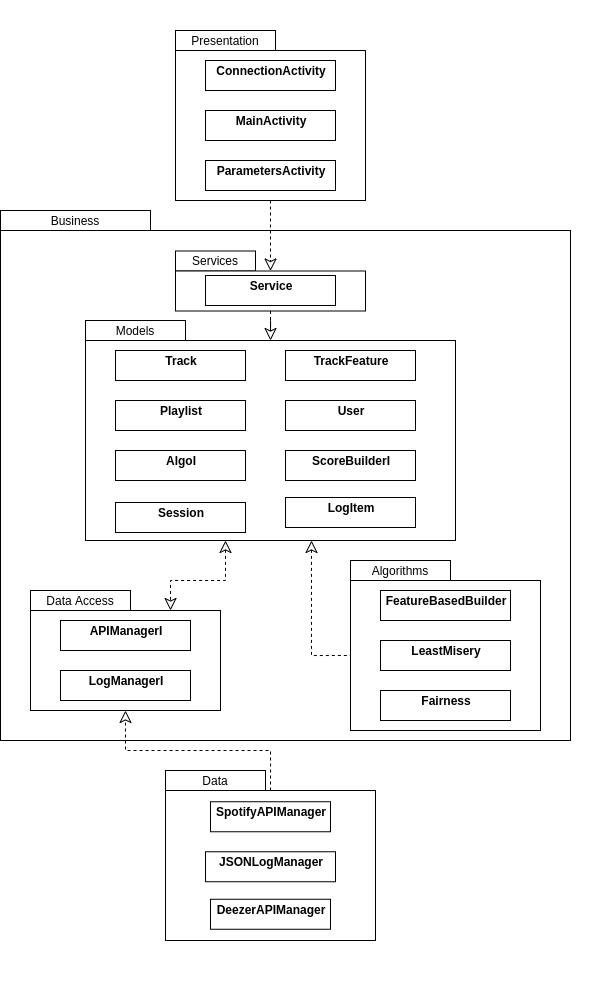
\includegraphics[scale=0.5]{ressources/diagramme_paquetage.png}
			\caption{Diagramme de paquetage de l'application}
			\label{fig:package_diag}
		\end{figure}
		\newpage
		Tout d'abord, pour avoir un haut niveau de granularité, nous avons imaginé une architecture en 3 couches (Figure \ref{fig:package_diag}. Celle-ci contient une couche "Présentation" qui correspond au côté Front. Elle contient les différentes pages de l'application. Cette couche communique avec la couche "Business" via une façade "Services" dont l'utilité est détaillée dans la sous-partie suivante (cf. \ref{class_diag}). Cette couche correspond à la partie métier, elle contient uniquement des concepts métiers tels que Playlist, User, Algorihmes, etc.. Elle contient aussi une partie "Data Access", qui comprend les interfaces des classes permettant d'écrire ou d'accéder à des données extérieures à l'application. C'est donc via cette sous-couche que la couche métier communique avec la couche "Data", dans laquelle on peut retrouver les implémentations de communication avec des API de services de streaming(Spotify, Deezer, ou autres), mais aussi l'implémentation de la gestion du Log (ici, au format JSON).
		\subsection{Diagramme de Classes}\label{class_diag}
		\paragraph{}
		Nous avons donné une grande importance à notre architecture de classes (Figure \ref{fig:class_diag}) de façon à permettre un maximum d'extension, mais aussi pour simplifier, le travail en équipe et la séparation des tâches. Ici, la classe Session est l'agrégat qui gère l'ensemble des autres classes. On peut observer un grand nombre d'interfaces (AlgoI, ScoreBuilderI, LogManager, APIManager) de façon à pouvoir, si besoin, ajouter des extensions à l'application. Par exemple, ajouter de nouveaux algorithmes, une autre façon d'écrire le log, ou  bien ajouter d'autres API de services de streaming. Le deuxième point majeur de notre architecture est la classe Service qui agit comme une façade avec le reste du code. De ce fait, cela permet de séparer complètement les tâches de Frontend et de Backend. En effet, les services sont appelés coté Front, ce qui permet à la partie de l'équipe concernée de ne pas se soucier de l'implémentation des méthodes appelées et de se concentrer sur la partie graphique uniquement.
		
		\newpage
		\begin{figure}[h!]
			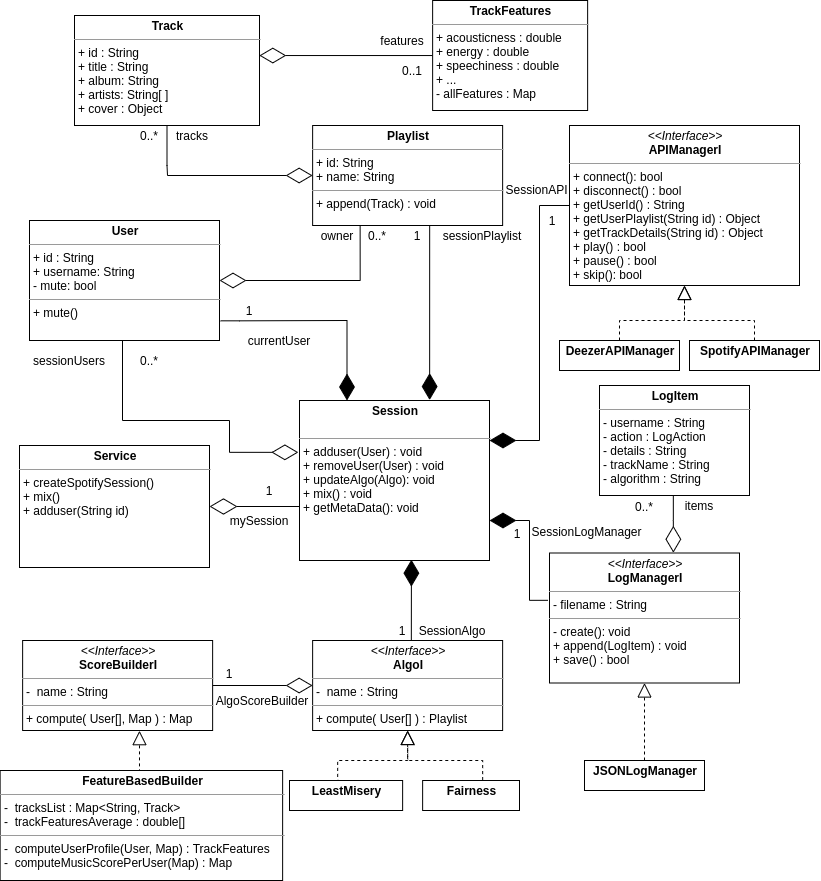
\includegraphics[width=\linewidth]{ressources/diagramme_classes.png}
			\caption{Diagramme de classes de l'application}
		\end{figure}
		
		\newpage
		
		\subsection{Architecture de l'application}\label{archi_log}
		\todo{TODO}
		\begin{figure}[h!]
			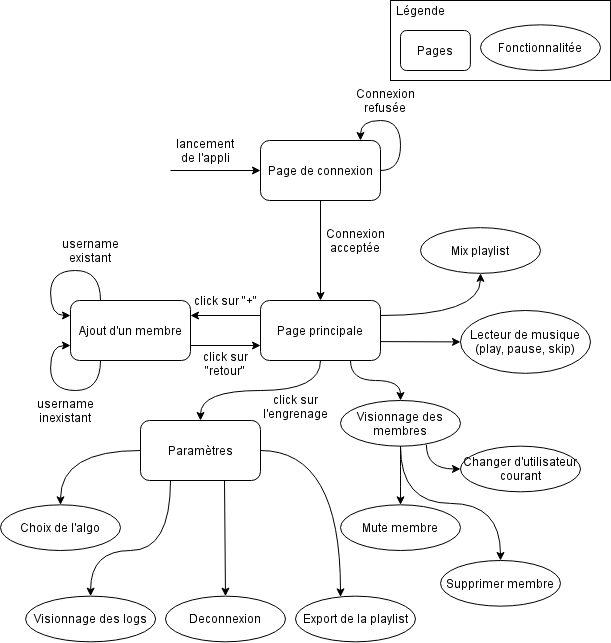
\includegraphics[width=\linewidth]{ressources/Architecture_Log.png}
			\caption{Architecture de l'application}
			\label{fig:class_diag}
		\end{figure}
	
	    \newpage
		\section{Analyse du fonctionnement et tests}
	
    	\todo{TODO analyse du fonctionnement du logiciel, description des tests et discussions de
        leurs résultats, explication des problèmes, défauts, et bugs.}

		\section{Conclusion}
        \todo{TODO description de ce qu’il y aurait encore à faire,
                extensions (et comment les réaliser).}
			
		\section{Bibliographie}
		\bibliography{references}
						
								
\end{document}